\section{Setup}
\subsection{Two-Body Problem}\label{two_body_problem}

The \textbf{hydrogen atom} is one of the most important problems in quantum mechanics. As the simplest of the atoms, it is the easiest to model, and the solutions can be used to consider larger atoms. In addition, it can be approached again and again at different levels. We conclude this course by solving the hydrogen atom using the methods we have learned so far.

The hydrogen atom consists of a \textbf{proton} with position $\mathbf{x}_p$ and momentum $\mathbf{p}_p$, and an \textbf{electron} with position $\mathbf{x}_e$ and momentum $\mathbf{p}_e$. These are \textit{canonical variables}, meaning they obey the commutation relations \begin{align*}[\mathbf{x}_{p_i},\mathbf{p}_{p_j}]&=i\hbar\delta_{ij}\\ [\mathbf{x}_{e_i},\mathbf{p}_{e_j}]&=i\hbar\delta_{ij}\end{align*}Here the subscripts $i,j=1,2,3$ denote the various components of the vector operators. Furthermore, the proton variables commute with the electron variables. That is, we have two pairs of \textit{independent} canonical variables.

The wavefunction for the system is a function $\Psi(\mathbf{x}_p,\mathbf{x_e})$ of the positions of both particles. The quantity $|\Psi(\mathbf{x}_p,\mathbf{x}_e)|^2\,d^3\mathbf{x}_p\,d^3\mathbf{x}_e$ represents the probability of finding the proton in a certain location \textit{and} the electron within a certain location. Then to find the probability of only finding the proton in a certain location, we simply integrate over all the possible locations of the electron.

\begin{framedrmk*}[Many-body systems]
    The ability of quantum mechanics to represent a system of many objects in a single wavefunction has led some physicists to speculate about a grand wavefunction of the entire universe.
\end{framedrmk*}

The Hamiltonian for the hydrogen atom is $$\hat{H}=\frac{(\mathbf{p}_p)^2}{2m_p}+\frac{(\mathbf{p}_e)^2}{2m_e}+V(|\mathbf{x}_e-\mathbf{x}_p|).$$Note that the kinetic energy is simply the sum of the kinetic energies of the two particles, and that the potential depends only on the magnitude of the separation between the particles.

In order to simplify the problem, we introduce two new pairs of independent canonical variables. The first pair is associated with the motion of the \textit{center of mass} of the system. Specifically, we introduce the total momentum operator $\hat{\mathbf{P}}$ and the center of mass position operator $\hat{\mathbf{X}}$, given by $$\hat{\mathbf{P}}=\hat{\mathbf{p}_p}+\hat{\mathbf{p}_e},\quad\quad\hat{\mathbf{X}}=\frac{m_e\hat{\mathbf{x}_e}+m_p\hat{\mathbf{x}}_p}{m_e+m_p}.$$Using the commutation relations above, we can show that $\hat{\mathbf{X}}$ and $\hat{\mathbf{P}}$ are canonical conjugates: $$[\hat{\mathbf{X}}_i,\hat{\mathbf{P}}_j]=i\hbar\delta_{ij}.$$For the second pair of canonical variables, we will define the \textit{relative} position and momentum operators. The relative position operator is defined naturally as $$\hat{\mathbf{x}}=\hat{\mathbf{x}}_e-\hat{\mathbf{x}}_p.$$We can check that $\hat{\mathbf{x}}$ commutes with both $\hat{\mathbf{X}}$ and $\hat{\mathbf{P}}$. We now construct a relative momentum operator that is a canonical conjugate of $\hat{\mathbf{x}}$. We write $$\hat{\mathbf{p}}=\alpha\hat{\mathbf{p}}_e-\beta\hat{\mathbf{p}}_p,$$where $\alpha$ and $\beta$ are constants to be determined. We must have $[\hat{\mathbf{x}}_i,\hat{\mathbf{p}}_j]=i\hbar\delta_{ij}$, which implies that $\alpha+\beta=1$. Additionally, the relative momentum must commute with the center of mass position, which implies that $m_e\alpha-m_p\beta=0$. These equations yield $$\alpha=\frac{m_p}{m_e+m_p},\qquad \beta=\frac{m_e}{m_e+m_p}.$$We also define the total mass $M=m_e+m_p$ and the **reduced mass** $\mu=\frac{m_em_p}{m_e+m_p}$. Then we have $\alpha=\frac{\mu}{m_e}$ and $\beta=\frac{\mu}{m_p}$. Thus, we can rewrite the relative momentum operator as $$\hat{\mathbf{p}}=\mu\bigg(\frac{\hat{\mathbf{p}}_e}{m_e}-\frac{\hat{\mathbf{p}}_p}{m_p}\bigg).$$Therefore, the relative momentum vanishes if the velocities of the two particles are the same.

We can now rewrite the Hamiltonian in terms of the new variables. Solving for the original momentum operators in terms of $\hat{\mathbf{P}}$ and $\hat{\mathbf{p}}$, we find $$\hat{\mathbf{p}}_p=\frac{m_p}{M}\hat{\mathbf{P}}-\hat{\mathbf{p}},\qquad\hat{\mathbf{p}}_e=\frac{m_e}{M}\hat{\mathbf{P}}+\hat{\mathbf{p}}.$$We can then rewrite the kinetic energy terms of the Hamiltonian in the form $$\frac{\hat{\mathbf{p}}_p^2}{2m_p}+\frac{\hat{\mathbf{p}}_e^2}{2m_e}=\frac{\hat{\mathbf{P}}^2}{2M}+\frac{\hat{\mathbf{p}}^2}{2\mu}.$$We see that the center of mass motion and the relative motion give independent contributions to the kinetic energy. The Hamiltonian can then be written as $$\hat{H}=\frac{\hat{\mathbf{P}}^2}{2M}+\frac{\hat{\mathbf{p}}^2}{2\mu}+V(\hat{\mathbf{x}}).$$

\subsection{Center of Mass and Relative Motion Wavefunctions}\label{com_relative_wavefunctions}

In position space, the total and relative momentum operators can be expressed as gradients: $$\hat{\mathbf{P}}=\frac{\hbar}{i}\nabla_X, \qquad\hat{\mathbf{p}}=\frac{\hbar}{i}\nabla_x.$$The subscripts indicate the system of coordinates with respect to which the gradient is taken. 

We solve the time-independent Schrödinger equation using separation of variables: $$\Psi(\mathbf{X},\mathbf{x})=\Psi_{CM}(\mathbf{X})\Psi_{rel}(\mathbf{x}).$$Plugging into the Schrödinger equation $\hat{H}\Psi=E\Psi$, $$\bigg[(\frac{\hat{\mathbf{P}}^2}{2M})\Psi_{CM}(\mathbf{X})\bigg]\Psi_{rel}(\mathbf{x})+\bigg[(\frac{\hat{\mathbf{p}}^2}{2\mu})\Psi_{rel}(\mathbf{x})+V(|\mathbf{x}|)\Psi_{rel}(\mathbf{x})\bigg]\Psi_{CM}(\mathbf{X})=E\Psi_{CM}(\mathbf{X})\Psi_{rel}(\mathbf{x}).$$This is very similar to the work we did in two dimensions, when we split the wavefunction into its dependence on $x$ and $y$. Dividing by the total wavefunction, $$\frac{1}{\Psi_{CM}(\mathbf{X})}(\frac{\hat{\mathbf{P}}^2}{2M})\Psi_{CM}(\mathbf{X})+\frac{1}{\Psi_{rel}(\mathbf{x})}\bigg[(\frac{\hat{\mathbf{p}}^2}{2\mu})\Psi_{rel}(\mathbf{x})+V(|\mathbf{x}|)\Psi_{rel}(\mathbf{x})\bigg]=E.$$The right-hand side is a constant. The left-hand side is the sum of two functions, the first of which depends only on the center-of-mass position $\mathbf{X}$ and the second of which depends only on the relative position $\mathbf{x}$. Therefore, both terms on the left-hand side must be equal to constants $E_{CM}$ and $E_{rel}$, respectively. This yields \begin{align*}(\frac{\hat{\mathbf{P}}^2}{2M})\Psi_{CM}(\mathbf{X}) =E_{CM}\Psi_{CM}(\mathbf{X}), \\  (\frac{\hat{\mathbf{p}}^2}{2\mu})\Psi_{rel}(\mathbf{x})+V(|\mathbf{x}|)\Psi_{rel}(\mathbf{x}) = E_{rel}\Psi_{rel}(\mathbf{x}), \\ E = E_{CM}+E_{rel}.\end{align*}We now have two Schrödinger equations. The first equation tells us that the center of mass moves as a free particle of mass $M$. Thus, the center of mass energy is not quantized and we get plane wave solutions. The second equation is for the relative motion of the electron and proton. It is described as motion in a central potential $V(|\mathbf{x}|)$. The third equation tells us that the total energy is the sum of the center of mass energy and the energy from relative motion. 

\subsection{Hydrogen Atom Potential}

We now have the tools to study the hydrogen atom, which has a central potential given by $$\boxed{V(r)=-\frac{Ze^2}{r},}$$where $Z$ is the number of protons in the nucleus. For hydrogen, we of course have $Z=1$, but we build in the flexibility to consider an electron orbiting the nucleus of some other atom. We first define a couple physical constants.

\begin{itemize}
    \item The \textbf{fine structure constant} $\alpha=\frac{e^2}{\hbar c}\approx\frac{1}{137}$.
    \item The \textbf{Bohr radius} $a_0$: the characteristic length scale in the problem, $a_0=\frac{\hbar^2}{me^2}\approx 53\,pm$.
\end{itemize}

There are some other characteristic quantities that are useful:

\begin{itemize}
    \item The energy scale estimate is $\frac{e^2}{a_0}\approx 27.2\,eV$.
    \item The Compton wavelength of the electron is $\alpha a_0\approx 390\,fm$.
    \item The classical electron radius is $\alpha^2 a_0\approx 2.8\,fm$.
\end{itemize}

\section{Energy Eigenstates of Hydrogen}
\subsection{Solving the Hydrogen Atom}\label{solving_hydrogen_atom}

We now solve for the bound states ($E<0$) of the hydrogen atom. Using the expression for the central potential, we can write the radial equation for hydrogen as $$\bigg(-\frac{\hbar^2}{2m}\frac{d^2}{dr^2}+\frac{\hbar^2l(l+1)}{2mr^2}-\frac{Ze^2}{r}\bigg)u(r)=Eu(r).$$Recall that the radial equation is derived from the Schrödinger equation by setting $\psi(r,\theta,\phi)=\frac{u(r)}{r}Y_{lm}(\theta,\phi)$. We wish to eliminate units, so we set $r=\frac{a_0}{2Z}x$, where $x$ is a unit-free proxy for radius. The factor of $Z$ serves to also cancel $Z$ in the radial equation.

The Schrödinger equation then becomes \begin{align*}\bigg(-\frac{\hbar^2}{2m}\frac{4Z^2}{a_0^2}\frac{d^2}{dx^2}+\frac{4Z^2}{a_0^2}\frac{\hbar^2l(l+1)}{2mx^2}-\frac{2Z^2e^2}{a_0}\frac{1}{x}\bigg)u&=Eu\\ \bigg(\frac{2\hbar^2Z^2}{ma_0^2}\bigg(-\frac{d^2}{dx^2}+\frac{l(l+1)}{x^2}\bigg)-\frac{2Z^2e^2}{a_0}\frac{1}{x}\bigg)u&=Eu. \end{align*}Note that $$\frac{2\hbar^2Z^2}{ma_0^2}=\frac{2\hbar^2Z^2}{ma_0}\frac{me^2}{\hbar^2}=\frac{2Z^2e^2}{a_0}.$$This reduces our equation to $$\bigg(-\frac{d^2}{dx^2}+\frac{l(l+1)}{x^2}-\frac{1}{x}\bigg)u=\frac{E}{(\frac{2Z^2e^2}{a_0^2})}u.$$We now define the unit-free parameter $\kappa$ that encodes the energy: $$\kappa^2=-\frac{E}{{(\frac{2Z^2e^2}{a_0})}}>0.$$The differential equation is then $$\bigg(-\frac{d^2}{dx^2}+\frac{l(l+1)}{x^2}-\frac{1}{x}\bigg)u=-\kappa^2 u.$$We can further simplify this equation by examining the limiting cases. As $x\to\infty$, the dominant term on the left is the second derivative, which gives $$\frac{d^2u}{dx^2}=\kappa^2 u\quad\implies\quad u\sim e^{\pm\kappa x}.$$Since $\kappa$ and $x$ are both dimensionless, we can introduce yet another unit-free parameter $\rho$ equal to the exponent above: $$\rho=\kappa x=\frac{2\kappa Z}{a_0}r.$$This time we get $$\boxed{\bigg(-\frac{d^2}{d\rho^2}+\frac{l(l+1)}{\rho^2}-\frac{1}{\kappa\rho}\bigg)u=-u.}$$Note that $\kappa$ has not completely disappeared. This is good news --- the equation should end up fixing the possible values of $\kappa$, which will correspond to the allowed values of $E$.

As $\rho\to\infty$, we now have that $u\sim e^{\pm\rho}$, and we of course hope for $u\sim e^{-\rho}$ for normalizability. In Section \ref{effective_potential}, we saw that as $\rho\to0$, $u\sim p^{l+1}$. This information suggests the following ansatz for $u(\rho)$: $$u(\rho)=\rho^{l+1}W(\rho)e^{-\rho},$$where $W(\rho)$ is a yet-to-be-determined function that we hope satisfies a simpler differential equation. Plugging this into the boxed equation and doing some messy algebra, we get $$\boxed{\rho\frac{d^2W}{d\rho^2}+2(l+1-\rho)\frac{dW}{d\rho}+[\frac{1}{\kappa}-2(l+1)]W=0.}$$Here we feel upset; the equation appears to be worse than the one we started with! However, it all leads to a very nice recursion relation.

As usual, we express $W(\rho)$ as a power series $W=\sum_{k=0}^\infty a_k\rho^k$ to find $a_{k+1}$ in terms of $a_k$. Some simple algebra yields $$\boxed{\frac{a_{k+1}}{a_k}=\frac{2(k+l+1)-\frac{1}{\kappa}}{(k+1)(k+2l+2)}.}$$Now for very large $k$, we have $$\lim_{k\to\infty}\frac{a_{k+1}}{a_k}=\frac{2}{k}>\frac{2}{k+1}.$$Therefore, if the series with common ratio $\frac{2}{k+1}$ diverges, so will the expansion of $W$. Thus we can bound the limiting behavior of $W$ with the series $a_{k+1}=\frac{2}{k+1}a_k$, which has closed form $$a_k=\frac{2^k}{k!}a_0.$$This produces $$W=\sum_{k=0}^\infty a_k\rho^k\lesssim a_0\sum_{k=0}^\infty\frac{2^k\rho^k}{k!}=a_0e^{2\rho}.$$Recall that our ansatz for $u$ was $$u(\rho)=\rho^{l+1}W(\rho)e^{-\rho}.$$Then if $W$ grows with $e^{2\rho}$, $u$ grows exponentially with $\rho$ and cannot be normalized. Therefore, the series expansion of $W$ must terminate --- $W$ must be a polynomial. Suppose $W$ has degree $N$: $a_N\neq 0$ and $a_{N+1}=0$. Since our recursion relation expresses $a_{k+1}$ as a multiple of $a_k$, all coefficients above $a_{N+1}$ would then be $0$ also.

From the boxed recursion relation, we have $$\frac{1}{\kappa}=2(N+l+1).$$Somehow, quantization has happened! We have related the energy parameter $\kappa$ to the integers! Note that $l$ can take any whole number value, as there are no constraints on the angular momentum of the system. Furthermore, $N$ can also take any whole number value, since a polynomial can have any whole number degree! We define the **principal quantum number** $n$ as follows: $$n=N+l+1=\frac{1}{2\kappa},$$with $l,N\in \mathbb{N}_0$ and $n\in\mathbb{N}$. Importantly, the energies depend only on $n$! By the definition of $$\kappa^2=-\frac{E}{(\frac{2Z^2e^2}{a_0^2})},$$we have $$E=-\frac{Z^2e^2}{2a_0}\frac{1}{n^2}.$$These are the energy levels of the hydrogen atom! Since at any value of $n>1$ there are numerous possible values of $l$, the spectrum is highly degenerate. 

\subsection{Hydrogen Atom Spectrum}\label{hydrogen_spectrum}

One way to visualize the spectrum of the hydrogen atom is shown in Figure \ref{hydrogen_spectrum}. All lattice points in the first quadrant of the $N$-$l$ plane represent states. The states with common value of $n$ lie on the diagonal lines.

\begin{figure}
    \centering
    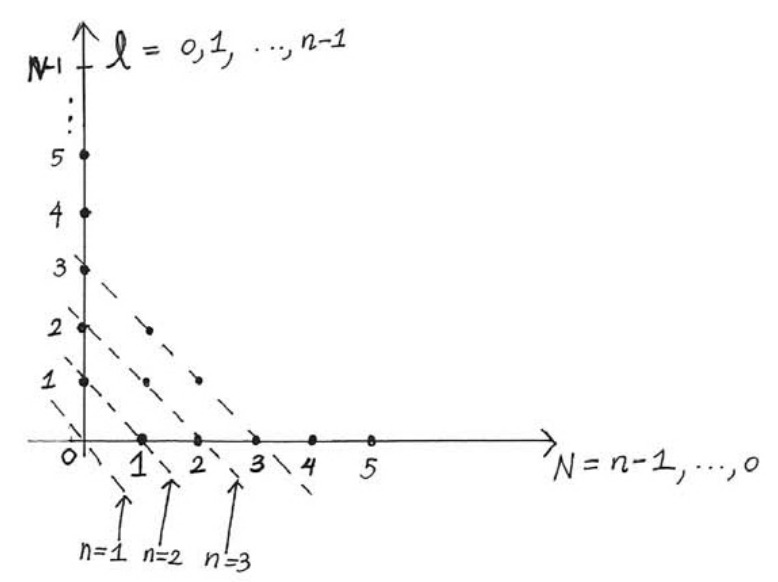
\includegraphics[width=0.5\linewidth]{resources/images/hydrogen_spectrum.png}
    \caption{A visualization of the spectrum of the hydrogen atom. States that share a dotted line are degenerate.}
    \label{hydrogen_spectrum}
\end{figure}

This figure helps us to count the number of bound states for a given value of $n$. Recall that $l$ can take values from $0$ to $n-1$, and for each value of $l$, the third quantum number $m$ can take the $(2l+1)$ values from $-l$ to $l$. Table \ref{hydrogen_spectrum} counts the states for the first three values of $n$. A state is specified by its values of $n$, $l$, and $m$, which are collectively referred to as the \textbf{quantum numbers} of the hydrogen atom. Each number has a very important physical meaning: $n$ specifies the energy eigenvalue, $\hbar^2 l(l+1)$ is the eigenvalue of the square of the angular momentum, and $\hbar m$ is the eigenvalue of the $z$-component of the angular momentum.

\begin{table}[]
    \centering
    \begin{tabular}{|c|c|c|c|}
    \hline
        $n$ & $l$ & $m$ & \# of states \\
        \hline
        $n=1$ & $l=1$ & $m=0$ & $1$ state \\
        \hline
        $n=2$ & $l=0$ & $m=1 $& $1$ \\
        & $l=1$ & $m=-1,0,1$ & $+3$ \\ 
        & & & $=4$ states \\
        \hline
        $n=3$ & $l=0$ & $m=0$ & $1$\\
        & $l=1$ & $m=-1,0,1$ & $+3$ \\
        & $l=2$ & $m=-2,\ldots,2$ & $+5$ \\
        & & & $=9$ states \\
    \hline
    \end{tabular}
    \caption{A table of the quantum numbers of the first few hydrogen atom eigenstates}
    \label{hydrogen_spectrum}
\end{table}

The total number of states for a given value of $n$ is $$\sum_{l=0}^{n-1}(2l+1)=\frac{2(n-1)n}{2}+n=n^2-n+n=n^2.$$Let us recap. Recall that way back at the beginning of our solution, we defined $\rho=\frac{2\kappa Z}{a_0}r$. But now we know what $\kappa$ is: $\kappa=\frac{1}{2n}$. This gives $$\rho=\frac{Z}{na_0}r.$$The wavefunctions are \begin{align*}\psi_{nlm}&=\mathcal{N}\frac{u_{nl}(r)}{r}Y_{lm}(\theta,\phi)=\mathcal{N}\frac{\rho^{l+1}}{\rho}W_{nl}(\rho)e^{-\rho}Y_{lm}(\theta,\phi)\\ &= \mathcal{N}\rho^l W_{nl}(\rho)e^{-\rho}Y_{lm}(\theta,\phi)\end{align*}where $\mathcal{N}$ is a normalization constant and $W_{nl}(\rho)$ is a polynomial of degree $N=n-l-1$. Substituting our expression for $\rho$ and absorbing constants into $N$, we have $$\boxed{\psi_{nlm}(r,\theta,\phi)=\mathcal{N}(\frac{r}{a_0})^l({\scriptstyle\text{polynomial in $\frac{r}{a_0}$ with degree $n-l-1$}})e^{-\frac{Zr}{na_0}}Y_{lm}(\theta,\phi)}.$$For the ground state of hydrogen, we have $Z=1$, $n=1$, $l=m=0$. Since there is no angular momentum, the associated wavefunction has no angular dependence. The normalized wavefunction is $$\psi_{100}(r,\theta,\phi)=\frac{1}{\sqrt{\pi a_0^3}}e^{-r/a_0}.$$For normalized wavefunctions of hydrogen with $n=1,2,3$, check out \href{http://hyperphysics.phy-astr.gsu.edu/hbase/quantum/hydwf.html}{this} website.

\begin{framedrmk*}
    What \textit{are} the mysterious polynomials $W_{nl}(\rho)$? They are known as the \textbf{associated Laguerre polynomials}, and more information about them can be found \href{https://en.wikipedia.org/wiki/Laguerre_polynomials#In_quantum_mechanics}{here}. They are quite interesting mathematical objects in their own right, but they are never necessary for any but the most precise calculations. 
\end{framedrmk*}

The canonical way of representing the energy levels of the hydrogen atom is shown in Figure \ref{hydrogen_energy_levels}. On the vertical axis we plot the possible values of $\frac{-1}{n^2}=\frac{2a_0E}{z^2e^2}$. Up to a proportionality constant, these represent the allowed energy levels. On the horizontal axis, we plot the possible values of $l$. 

\begin{figure}
    \centering
    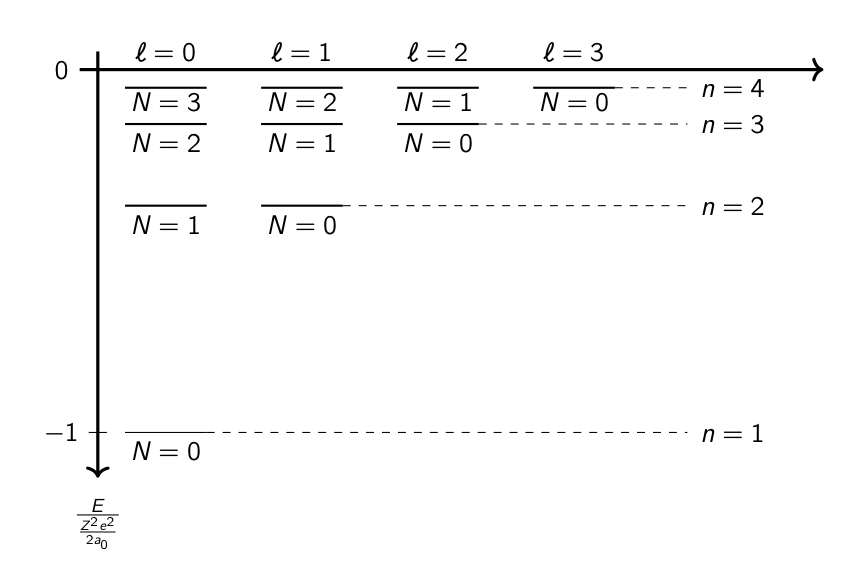
\includegraphics[width=0.5\linewidth]{resources/images/hydrogen_atom_energ_levels.png}
    \caption{A diagram of the energy levels of the hydrogen atom.}
    \label{hydrogen_energy_levels}
\end{figure}

As shown, the values of $N$ are constant along the diagonals, and increasing vertically. Why is this? Recall that for a constant value of $l$, the solutions obey a radial wave equation and thus the node theorem. Since all the nodes must come from the radial Laguerre polynomials, the polynomials must have degree increasing with $n$. Thus, $N$ must increase with $n$ to allow for more roots.

\subsection{Features of the Solutions}\label{features_of_the_solution}

It is important to note the extraordinary degeneracy within the hydrogen atom eigenstates. It is entirely unclear why $N=0$ eigenstates, for example, would be degenerate with $N=1$ eigenstates. In fact, the seemingly more simple system of the infinite spherical well has no degeneracies. The repeated eigenvalues of the hydrogen atom are a hint at a deeper symmetry that we are not yet aware of. We will explore this hidden symmetry in the coming sections.

We begin by rewriting the ground state wavefunction for the hydrogen atom, with $Z=1$ protons: $$\psi_{100}=\frac{1}{\sqrt{\pi a_0^3}}e^{-{r/a_0}}.$$We may ask how this wavefunction would change for $Z\neq 1$. Recall that the potential is $V(r)=-\frac{ze^2}{r}$. Then if $e^2$ becomes $Ze^2$, we can reason that $a_0=\frac{\hbar}{me^2}$ would become $\frac{a_0}{Z}$. Recall that $$E=-\frac{Z^2e^2}{2a_0}\frac{1}{n^2}.$$We can now see that one factor of $Z$ arises from the $e^2$ in the numerator, and the other factor is due to the $a_0$ in the denominator.

The general ground state wavefunction for an atom with $Z$ protons then becomes $$\psi_{100}=\sqrt{\frac{Z^3}{\pi a_0^3}}e^{-\frac{Zr}{a_0}}.$$We might also ask about the reason for the exponential $e^{-\frac{Zr}{na_0}}$ in the expression for the wavefunctions. Recall that we obtain the limiting case $$\frac{d^2u}{dr^2}=-\frac{2mE}{\hbar^2}u.$$The energy levels obey $$E_n=-\frac{Z^2e^2}{2a_0}\frac{1}{n^2}=-\frac{Z^2}{2a_0}\frac{\hbar^2}{ma_0}\frac{1}{n^2}.$$Therefore, $$-\frac{2mE_n}{\hbar^2}=\frac{Z^2}{n^2a_0^2}.$$Substituting, we have $$\frac{d^2u}{dr^2}=\frac{Z^2}{n^2a_0^2}u,$$which is solved by the exponential $$u(r)=e^{-\frac{Zr}{na_0}}.$$

\subsection{Rydberg Atoms}\label{rydberg_atoms}

A \textbf{Rydberg atom} is one in which one or more electrons is in a very high energy state. This leads to several unique properties. The outermost electron feels the attractive field due to the positive charge $Ze$ of the protons, but also the repulsive field due to the negative charge $(Z-1)e$ of the other electrons. Thus in any Rydberg atom, the outermost electron behaves as an electron in a hydrogen atom. One interesting question is the size (expected radius) of a Rydberg atom. To consider this, we state the \textbf{virial theorem}, an important result from statistical mechanics.

\begin{framedthm}[Virial theorem]
    For any particle in a potential $V$ with kinetic energy $T$, it is always true that $\langle T\rangle = -\frac{1}{2}\langle V\rangle$. In other words, $E=-\langle T\rangle$ and $\langle V\rangle=2E$.
\end{framedthm}

For a Rydberg atom (where we consider $Z=1$), the virial theorem gives $$\langle -\frac{e^2}{r}\rangle=2(-\frac{e^2}{2a_0}\frac{1}{n}).$$Simplifying, $$\langle\frac{1}{r}\rangle=\frac{1}{n^2 a_0}.$$Of course, the expectation value of $r$ is not the same as the reciprocal of the expected value of $\frac{1}{r}$. Instead, it turns out to be $$\langle r\rangle= n^2a_0[1+\frac{1}{2}(1-\frac{l(l+1)}{n^2})].$$Thus we see that the expected radius of a Rydberg atom does depend on $l$, but only very weakly. For $l=0$, we have $\langle r\rangle=\frac{3}{2}n^2a_0$, while for $l\to\infty$, we have $\langle r\rangle\approx n^2a_0$. 

Recall that the wavefunctions of the hydrogen atom are $$\psi_{nlm} = \mathcal{N}r^l W_{nl}(r)e^{-\frac{r}{na_0}}Y_{lm}(\theta,\phi)=f_{nl}(r)Y_{lm}(\Omega).$$We see that the exponential possesses a characteristic radius of $na_0$. Why is it, therefore, that the actual expected radius increases with $n^2$? We know that the probability $P(r)$ of finding the electron at a radius $r$ obeys $$P(r)dr=d^3x\,|\psi|^2=r^2dr\int d\Omega\,|\psi|^2=r^2dr\,|f_{nl}|^2\int d\Omega\,Y_{lm}^*Y_{lm}.$$The spherical harmonics are normalized, so we simply get $$P(r)=r^2|f_{nl}|^2.$$Let's expand $$f_{nl}(r)\sim r^l(a_0+\ldots+a'r^{n-l-1})e^{-r/na_0}.$$Since we're considering.a Rydberg atom, we can reason that the radius will be reasonably large. Thus, we keep only the term with highest degree in $r$: $$f_{nl}(r)\sim r^{n-1}e^{-r/na_0}.$$Therefore, the radial probability distribution obeys$$P(r)\sim r^{2n}e^{-\frac{2r}{na_0}}.$$We can see that there is a fight between an exponential with a characteristic width proportional to $na_0$, and a polynomial whose growth rate is dependent on $n$. We can find the maximum of this distribution by taking the derivative and setting it to $0$: $$(\frac{2n}{r}-\frac{2}{na_0})r^{2n}e^{-\frac{2r}{na_0}}=0.$$This implies that $\frac{2n}{r}=\frac{2}{na_0}$, which is solved when $$r=n^2a_0.$$Thus, the behavior of the probability distribution is directly dependent on $n^2$, not $n$. 

Interstellar hydrogen atoms can have immense energies; astrophysicists have observed electrons with $n$ as large as $350$! Using the expression we found above, we would expect such an atom to have radius $$r=a_0(350)^2=(0.53\times 10^{-10}\,\text{m})(350)^2\approx 6.5\,\mu\text{m}.$$This is an enormous atom! For contrast, a red blood cell has radius $8\mu\text{m}$. However, they do not decay as quickly as you might think. Energy levels characterized by $\frac{1}{n^2}$ have differences proportional to $\frac{1}{n^3}$. There are a lot of energy levels close together! Decaying from each to the next takes the atom up to a second.

\section{Degeneracies of the Hydrogen Atom}
\subsection{Hydrogen Atom Orbits}\label{hydrogen_orbits}

Consider an electron with $l=0$, and another electron with $l=99$. Which electron would have the most circular orbit? Although we often associate low $l$ with circular orbits, the $l=0$ electron actually has the most elliptical orbit, and the $l=99$ electron is the most circular. Why is this? Recall that the effective potential of the electron is $$\frac{\hbar l(l+1)}{2mr^2}-\frac{e^2}{r}.$$If $l=0$, the potential goes purely with $-\frac{1}{r}$. Classically,  the electron's radius would oscillate between $r=0$ and some maximum value $r'$. However, this is the definition of the most eccentric orbit!

As $l$ increases, the graphs of the potential have higher and higher minima, as shown in Figure \ref{hydrogen_potential_graph}. At some point, the minimum of the potential lies exactly on the energy of the electron. This corresponds to an orbit with fixed orbit --- a circle. 

\begin{figure}
    \centering
    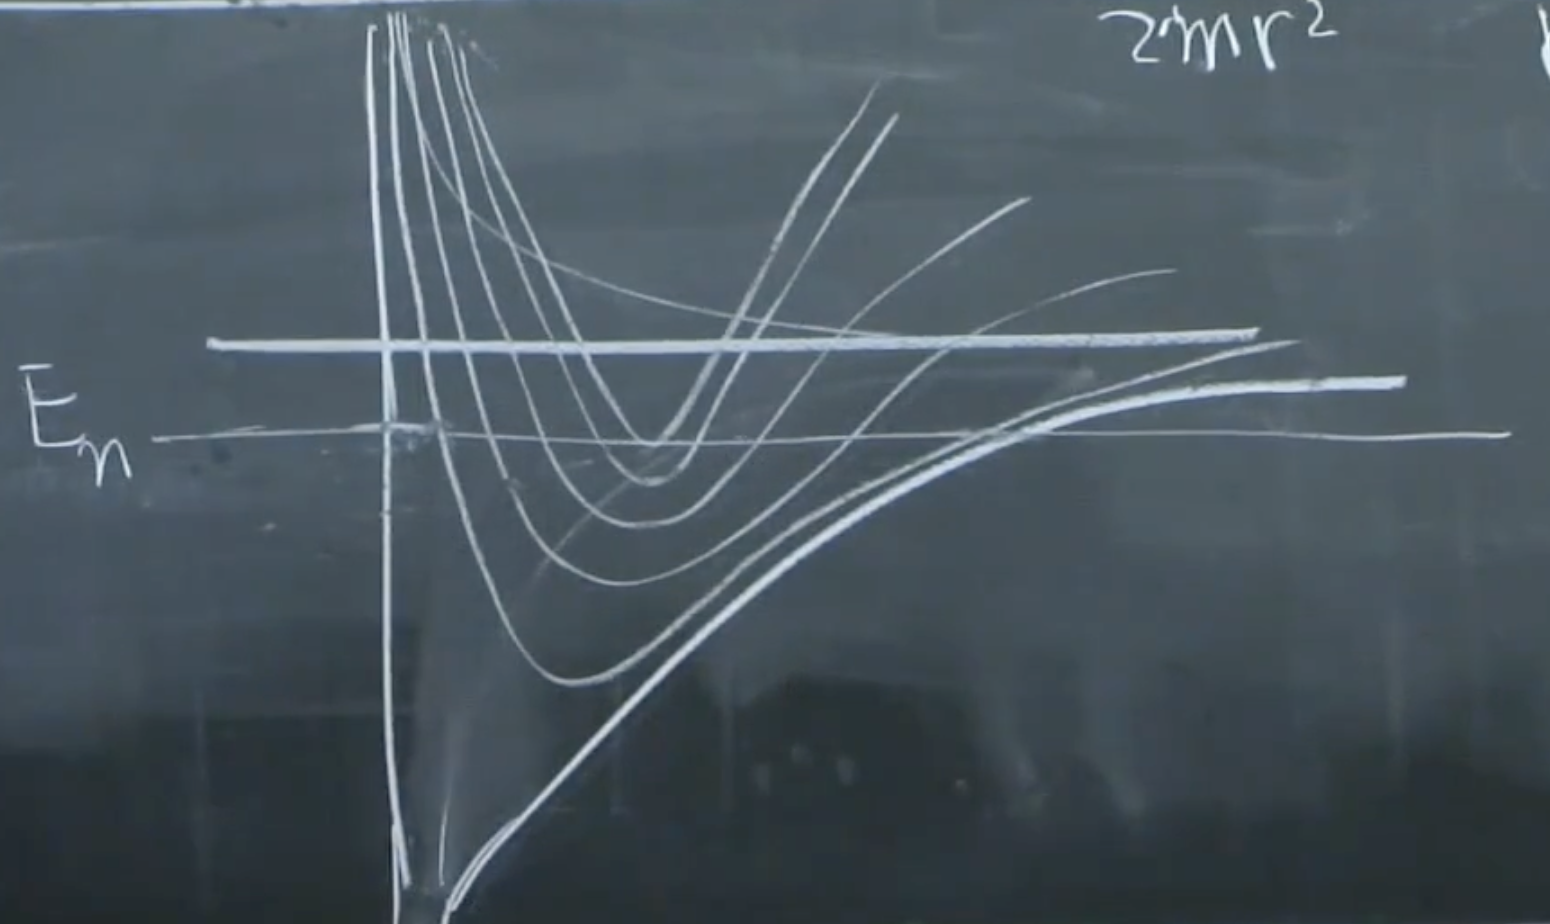
\includegraphics[width=0.5\linewidth]{resources/images/hydrogen_potential_graph.png}
    \caption{A graph of the potentials $V(r)$ for the hydrogen atom with differing values of $l$. As $l$ increases, the potentials have higher and higher minima.}
    \label{hydrogen_potential_graph}
\end{figure}

For any lower value of $l$, there exist two intersections between the effective potential and the energy value of the electron. These correspond to the two turning points of radius $r_-$ and $r_+$, respectively, as shown in Figure \ref{turning_points}. 

\begin{figure}
    \centering
    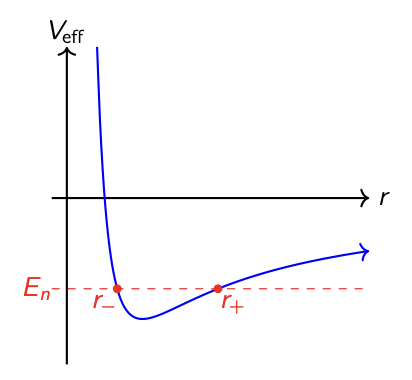
\includegraphics[width=0.5\linewidth]{resources/images/turning_points.png}
    \caption{A graph of the potential for some value of $l$. The two marked points are the turning points of radius $r_-$ and $r_+$, respectively.}
    \label{turning_points}
\end{figure}

\subsection{Turning Points}\label{turning_points_section}

We now solve explicitly for $r_-$ and $r_+$. We have $$V_{\text{eff}}(r)=\frac{\hbar^2 l(l+1)}{2mr^2}-\frac{e^2}{r}=E_n=-\frac{e^2}{2a_0}\frac{1}{n^2}$$at these turning points. We let $r=a_0x$, where $x$ is a unitfree length variable. This yields $$\frac{\hbar^2l(l+1)}{2ma_0^2}\frac{1}{x^2}-\frac{e^2}{a_0x}=-\frac{e^2}{2a_0}\frac{1}{n^2}.$$Also recall that $a_0=\frac{\hbar^2}{me^2}$, which gives $$\frac{\hbar^2}{2ma_0^2}=\frac{e^2}{2a_0}.$$Substituting, $$\frac{l(l+1)}{2a_0}\frac{1}{x^2}-\frac{e^2}{a_0x}=-\frac{e^2}{2a_0}\frac{1}{n}.$$Simplifying, $$\boxed{\frac{l(l+1)}{x^2}-\frac{2}{x}+\frac{1}{n^2}=0}.$$This is a quadratic in $\frac{1}{x}$. Multiplying both sides by $x^2$ gives us a quadratic in $x$. Solving, we get $$x=n^2\bigg(1\pm\sqrt{1-\frac{l(l+1)}{n^2}}\bigg).$$This yields $$r_\pm=n^2a_0\bigg(1\pm\sqrt{1-\frac{l(l+1)}{n^2}}\bigg).$$Recall that $l$ ranges from $0$ to $n$. When $l$ is very small, the orbit is extremely elliptical, as $r_\pm\approx n^2a_0(1\pm1)$. On the other hand, if $l$ is very large, the orbit is approximately circular: $r_\pm\approx n^2a_0$. Regardless of $l$, we see that $$\frac{1}{2}(r_-+r_+)=n^2a_0.$$

\begin{framedexpl}[Rydberg atom with $n=100$ and $l=60$]
    For $n=100$ and $l=60$, we have $r_+=18000a_0$, $r_-=2000a_0$.

\end{framedexpl}

Since the length of the semimajor axis of the orbit depends only on $n$, Kepler's third law tells us orbits with equal $n$ have equal periods. We know that periods are related to frequencies and thus energies, which explains why quantum states with equal $n$ are degenerate.

Lastly, consider a particular state with $l=1$. Then there are actually 3 degenerate states with this property: $m=-1$, $m=0$, and $m=1$. We don't represent these in our figures, but it should be noted that these degeneracies are always underlying.